% for notes environment
\usepackage{xsavebox}
\usepackage{hyperref}
\usepackage{graphicx}
\usepackage{luatexja}
\usepackage[hiragino-pro,deluxe,nfssonly,jis2004]{luatexja-preset}
\usepackage{fontspec}
\usepackage{epigraph}
\usepackage{etoolbox}
\usepackage{tikz}
\usepackage{framed}
\usepackage{mathtools}
\usepackage{listings}
\usepackage{libertine}
\usepackage[libertine]{newtxmath}
\usepackage{bxcoloremoji}
\usepackage{xcolor}
\usepackage{diagbox}
\usepackage{caption}
\usepackage{appendixnumberbeamer}
\usepackage{multirow}
\usepackage{xpatch}
\usepackage{multicol}
\usepackage{tabularx}
\usepackage{braket}
\usepackage{blochsphere}
\usepackage{bxtexlogo}
\bxtexlogoimport{SATySFi}

\usetikzlibrary{fit}

\setmonofont{CMU Typewriter Text}

\definecolor{links}{HTML}{2A1B81}
\hypersetup{colorlinks,linkcolor=,urlcolor=links}

\usetheme{Boadilla}
\usecolortheme{seahorse}
% \usefonttheme{serif}


\xpatchcmd{\itemize}
  {\def\makelabel}
  {\ifnum\@itemdepth=1\relax
     \setlength\itemsep{1.2ex}% separation for first level
   \else
     \ifnum\@itemdepth=2\relax
       \setlength\itemsep{0.8ex}% separation for second level
       \setlength\topsep{1.2ex}
     \else
       \ifnum\@itemdepth=3\relax
         \setlength\itemsep{0.05ex}% separation for third level
         \setlength\topsep{0.8ex}
   \fi\fi\fi\def\makelabel
  }
 {}
 {}

\setbeamercolor{page number in head/foot}{bg=blue!10}
\setbeamertemplate{footline}{%
  \leavevmode%
  \hbox{%
    \begin{beamercolorbox}[wd=.3\paperwidth,ht=2.25ex,dp=1ex,center]{author in head/foot}%
      \usebeamerfont{author in head/foot}\insertshortauthor\hspace*{1ex}(\insertshortinstitute)
    \end{beamercolorbox}%
    \begin{beamercolorbox}[wd=.2\paperwidth,ht=2.25ex,dp=1ex,center]{title in head/foot}%
      \usebeamerfont{title in head/foot}\insertshorttitle
    \end{beamercolorbox}%
    \begin{beamercolorbox}[wd=.4\paperwidth,ht=2.25ex,dp=1ex,center]{date in head/foot}%
      \insertshortdate{} @ \InsertConference
    \end{beamercolorbox}%
    \begin{beamercolorbox}[wd=.1\paperwidth,ht=2.25ex,dp=1ex,center]{page number in head/foot}%
      \insertframenumber{} / \inserttotalframenumber\hspace*{1ex}
    \end{beamercolorbox}}%
  \vskip0pt%
}

\beamertemplatenavigationsymbolsempty

\setbeamertemplate{bibliography item}{\insertbiblabel}
\setbeamersize{description width=1cm}
\setbeamertemplate{items}[circle]
\setbeamertemplate{section in toc}[circle]
\setbeamertemplate{subsection in toc}{%
  \leavevmode\leftskip=2em
  {%
    \usebeamerfont*{itemize item}%
    \usebeamercolor{subsection number projected}%
    \color{bg}%
    \raise1.25pt\hbox{\donotcoloroutermaths$\bullet$}}%
  \hskip1.5ex\inserttocsubsection\par}

% Definitions for the title page
\newcommand*{\GitHub}[1]{%
  \gdef\InsertGitHub{#1}%
}
\newcommand*{\Email}[1]{%
  \gdef\InsertEmail{\href{mailto:#1}{#1}}%
}
\newcommand*{\Conference}[1]{%
  \gdef\InsertConference{#1}%
}
\setbeamerfont{title}{size=\huge, series=\bfseries, family=\mcfamily\rmfamily}
\setbeamercolor{title}{bg=white}
\setbeamerfont{subtitle}{size=\small, series=\mdseries, family=\mcfamily\rmfamily}%\gtfamily\sffamily}
\setbeamerfont{email}{size=\scriptsize, family=\ttfamily}
\setbeamercolor{email}{bg=white}
\setbeamerfont{date}{shape=\itshape, family=\rmfamily}
\setbeamerfont{vc}{size=\scriptsize, family=\ttfamily}
\setbeamercolor{vc}{bg=white}

\renewcommand{\figurename}{Fig}

\input{vc.tex}

\setbeamertemplate{title page}
{%
  \vbox{}
  \vfill
  \begingroup
    \centering
    \hrulefill\par%
    \vskip1ex\par%
    \begin{beamercolorbox}[sep=0pt,center,shadow=false,rounded=true]{title}
      \vfill
      \usebeamerfont{title}\inserttitle\par%
      \ifx\insertsubtitle\@empty%
      \else%
        \vskip0.5ex%
        {\usebeamerfont{subtitle}\usebeamercolor[fg]{subtitle}\insertsubtitle\par}%
      \fi%
      \vfill  
    \end{beamercolorbox}%
    \hrulefill\par%
    \vskip2ex%
    \begin{beamercolorbox}[sep=0pt,center,shadow=false,rounded=true]{author}
      \usebeamerfont{author}\insertauthor
    \end{beamercolorbox}
    \begin{beamercolorbox}[sep=0pt,center,shadow=false,rounded=true]{email}
      \usebeamerfont{email}\InsertEmail
    \end{beamercolorbox}
    \vskip0.1ex
    \begin{beamercolorbox}[sep=5pt,center,shadow=false,rounded=true]{institute}
      \usebeamerfont{institute}\insertinstitute
    \end{beamercolorbox}
    \begin{beamercolorbox}[sep=5pt,center,shadow=false,rounded=true]{date}
      \usebeamerfont{date}\insertdate \normalfont @ \InsertConference
    \end{beamercolorbox}
    \begin{beamercolorbox}[sep=0pt,center,shadow=false,rounded=true]{vc}
      \usebeamerfont{vc}
      \url{https://github.com/\InsertGitHub} (\texttt{\GITAbrHash})
    \end{beamercolorbox}
    % {\centering
    %   \href{https://creativecommons.org/licenses/by-nc/4.0/}{%
    %     \includegraphics[width=0.1\textwidth]{img/by-nc.pdf}%
    %   }%
    % }
    {\usebeamercolor[fg]{titlegraphic}\inserttitlegraphic\par}
  \endgroup
  \vfill
}
\setbeamertemplate{blocks}[rounded][shadow=false]

% ============ ここを消すとNote消える ================
% \mode<handout>{%
%   \usepackage{pgfpages}
%   \setbeameroption{show notes on second screen=right}
%   \setbeamertemplate{note page}{%
%     \vspace{2ex}\insertnote%
%   }
% }
% ============ ここを消すとNote消える ================


\renewcommand{\kanjifamilydefault}{\gtdefault}

\setbeamertemplate{caption}[numbered]
\resetcounteronoverlays{lstlisting}
\definecolor{bluegray}{rgb}{0.4, 0.6, 0.8}
\DeclareCaptionFormat{listing}{{\color{bluegray}\lstlistingname}#2#3}
\captionsetup[lstlisting]{format=listing, font={footnotesize}}
\captionsetup[figure]{name={図}}
\captionsetup[table]{name={表}}
\setbeamerfont{footnote}{size=\scriptsize}

\setmonofont[Ligatures=TeX]{CMU Typewriter Text}

\setbeamertemplate{items}[circle]

\newfontfamily\quotefont[Ligatures=TeX]{Linux Libertine O} % selects Libertine as the quote font

\newcommand*\quotesize{60} % if quote size changes, need a way to make shifts relative
% Make commands for the quotes
\newcommand*{\openquote}{%
  \tikz[remember picture,overlay,xshift=0em,yshift=-3ex]
  \node (OQ) {\quotefont\fontsize{\quotesize}{\quotesize}\selectfont``};\kern0pt%
  \par\quad\par
}

\newcommand*{\closequote}[1]
  {\tikz[remember picture,overlay,xshift=1ex,yshift={#1}]
   \node (CQ) {\quotefont\fontsize{\quotesize}{\quotesize}\selectfont''};}

\newcommand*\shadedauthorformat{\emph} % define format for the author argument

% Now a command to allow left, right and centre alignment of the author
\newcommand*\authoralign[1]{%
  \if#1l
    \def\authorfill{}\def\quotefill{\hfill}
  \else
    \if#1r
      \def\authorfill{\hfill}\def\quotefill{}
    \else
      \if#1c
        \gdef\authorfill{\hfill}\def\quotefill{\hfill}
      \else\typeout{Invalid option}
      \fi
    \fi
  \fi}
% wrap everything in its own environment which takes one argument (author) and one optional argument
% specifying the alignment [l, r or c]
%
\newenvironment{shadequote}[2][l]%
{\hspace{0.5ex}
\authoralign{#1}
\ifblank{#2}
   {\def\shadequoteauthor{}\def\yshift{-1ex}\def\quotefill{\hfill}}
   {\def\shadequoteauthor{\par\authorfill\shadedauthorformat{#2}}\def\yshift{3ex}}
\begin{quote}\normalfont\openquote}
{\shadequoteauthor\quotefill\closequote{\yshift}\end{quote}}

\makeatletter
\def\@fnsymbol#1{\ensuremath{\ifcase#1\or \dagger\or \ddagger\or
   \mathsection\or \mathparagraph\or \|\or **\or \dagger\dagger
   \or \ddagger\ddagger \else\@ctrerr\fi}}
\makeatother

\renewcommand{\thefootnote}{\fnsymbol{footnote}}
\renewcommand{\thempfootnote}{\fnsymbol{mpfootnote}}
\newcommand\ballcircle[1]{%
  {%
    \usebeamercolor{enumerate item}%
    \tikzset{beameritem/.style={circle,inner sep=0,minimum size=2ex,text=enumerate item.bg,fill=enumerate item.fg}}%
    \tikz[baseline=(n.base)]\node(n)[beameritem]{\sffamily#1};%
  }%
}
\newcommand\ballref[1]{%
  \ballcircle{\ref{#1}}%
}

\usetikzlibrary{calc}
\usetikzlibrary{shapes.callouts} 

\pgfkeys{%
    /calloutquote/.cd,
    width/.code                   = {\def\calloutquotewidth{#1}},
    position/.code                = {\def\calloutquotepos{#1}}, 
    author/.code                  = {\def\calloutquoteauthor{#1}},
    at/.code                      = {\def\calloutquoteat{#1}},
    sign/.code                    = {\def\calloutquotesign{#1}},
    /calloutquote/.unknown/.code  = {\let\searchname=\pgfkeyscurrentname
                                      \pgfkeysalso{\searchname/.try=#1,                        
                                      /tikz/\searchname/.retry=#1},\pgfkeysalso{\searchname/.try=#1,
                                      /pgf/\searchname/.retry=#1}
                                    }
}

\makeatletter

\newsavebox\temp@simple@callout@author@box
\newcommand\calloutquote[2][]{%
  \pgfkeys{/calloutquote/.cd,
    width    = 5cm,
    position = {(0.5,-0.2)},
    at       = {(0,0)},
    author   = {},
    sign     = {+}
  }%
  \pgfqkeys{/calloutquote}{#1}%
  \sbox{\temp@simple@callout@author@box}{\mbox{%
    \begin{tabular}{l}
      \calloutquoteauthor%
    \end{tabular}
  }}%
  \node[thin, draw=black!50, rectangle callout,callout relative pointer={\calloutquotepos},align=center,text width=\calloutquotewidth,/calloutquote/.cd,
     #1] (tmpcall) at \calloutquoteat {#2};
  \node at ($ (tmpcall.pointer) - (-\calloutquotesign0.5\wd\temp@simple@callout@author@box,0.7\ht\temp@simple@callout@author@box) $) {\calloutquoteauthor};
}

\newsavebox\temp@simple@callout@box
\newcommand{\simplecallout}[4][{}]{%
  \sbox{\temp@simple@callout@box}{\mbox{%
    \begin{tabular}{l}
      #4%
    \end{tabular}
  }}%
  \begin{center}%
    \begin{tikzpicture}%
      \calloutquote[width=1.05\wd\temp@simple@callout@box,position={(#2.5,-0.2)},fill=#3,rounded corners,author={#1},sign=#2]{
        #4%
      }%
    \end{tikzpicture}%
  \end{center}
}

\makeatother
\newfontfamily{\listingfont}[Scale=0.85]{Menlo}
\definecolor{dkgreen}{rgb}{0,0.6,0}
\definecolor{gray}{rgb}{0.5,0.5,0.5}
\definecolor{mauve}{rgb}{0.58,0,0.82}

\makeatletter
\lst@CCPutMacro\lst@ProcessOther {"2D}{\lst@ttfamily{-{}}{-{}}}
\@empty\z@\@empty
\makeatother

\lstdefinestyle{csharp}{
  numbers=left,
  language=[Sharp]C
}

\lstdefinestyle{cil}{
  numbers=left,
  language=CIL
}

\lstdefinestyle{plain}{
  basicstyle=\listingfont\scriptsize,
  language=Plain,
  showstringspaces=false,
  showtabs=false,
  stringstyle=\listingfont\scriptsize\color{mauve},
  tabsize=2
}

\lstdefinestyle{sh}{
  numbers=left,
  language=sh
}

\lstdefinestyle{c}{
  numbers=left,
  language=C
}

\lstdefinestyle{python}{
  numbers=left,
  language=Python
}

\lstdefinestyle{asm-x86}{
  numbers=left
}

\lstdefinestyle{pseudo-code}{
  numbers=left,
  keywords=[6]{for,from,to,endfor,while,endwhile}
}

\lstdefinestyle{bitcoin-script}{
  mathescape=true
}

\lstset{
  basicstyle=\listingfont,
  frame=single,
  xleftmargin=2em,
  xrightmargin=1em,
  breaklines=true
}

\lstdefinestyle{scala}{
  basicstyle=\listingfont\scriptsize,
  breakatwhitespace=false,
  language=scala,
  captionpos=b,
  commentstyle=\listingfont\scriptsize\color{dkgreen},
  extendedchars=true,
  xleftmargin=1em,
  xrightmargin=1em,
  keepspaces=true,
  keywordstyle=\listingfont\scriptsize\color{blue},
  emphstyle=\listingfont\scriptsize\color{cyan},
  rulecolor=\listingfont\scriptsize\color{black},
  showspaces=false,
  showstringspaces=false,
  showtabs=false,
  stringstyle=\listingfont\scriptsize\color{mauve},
  tabsize=2
}

\lstdefinestyle{go}{
  basicstyle=\listingfont\scriptsize,
  breakatwhitespace=false,
  language=go,
  captionpos=b,
  commentstyle=\listingfont\scriptsize\color{dkgreen},
  extendedchars=true,
  xleftmargin=1em,
  xrightmargin=1em,
  keepspaces=true,
  keywordstyle=\listingfont\scriptsize\color{blue},
  emphstyle=\listingfont\scriptsize\color{cyan},
  rulecolor=\listingfont\scriptsize\color{black},
  showspaces=false,
  showstringspaces=false,
  showtabs=false,
  stringstyle=\listingfont\scriptsize\color{mauve},
  tabsize=2
}

\lstdefinestyle{js}{
  basicstyle=\listingfont\scriptsize,
  breakatwhitespace=false,
  language=JavaScript,
  captionpos=b,
  commentstyle=\listingfont\scriptsize\color{dkgreen},
  extendedchars=true,
  xleftmargin=1em,
  xrightmargin=1em,
  keepspaces=true,
  keywordstyle=\listingfont\scriptsize\color{blue},
  emphstyle=\listingfont\scriptsize\color{cyan},
  rulecolor=\listingfont\scriptsize\color{black},
  showspaces=false,
  showstringspaces=false,
  showtabs=false,
  stringstyle=\listingfont\scriptsize\color{mauve},
  tabsize=2
}

\lstdefinestyle{css}{
  basicstyle=\listingfont\scriptsize,
  breakatwhitespace=false,
  language=CSS,
  captionpos=b,
  commentstyle=\listingfont\scriptsize\color{dkgreen},
  extendedchars=true,
  xleftmargin=1em,
  xrightmargin=1em,
  keepspaces=true,
  keywordstyle=\listingfont\scriptsize\color{blue},
  emphstyle=\listingfont\scriptsize\color{cyan},
  rulecolor=\listingfont\scriptsize\color{black},
  showspaces=false,
  showstringspaces=false,
  showtabs=false,
  stringstyle=\listingfont\scriptsize\color{mauve},
  tabsize=2
}

\lstdefinestyle{html}{
  basicstyle=\listingfont\scriptsize,
  breakatwhitespace=false,
  language=HTML5,
  captionpos=b,
  commentstyle=\listingfont\scriptsize\color{dkgreen},
  extendedchars=true,
  xleftmargin=1em,
  xrightmargin=1em,
  keepspaces=true,
  keywordstyle=\listingfont\scriptsize\color{blue},
  emphstyle=\listingfont\scriptsize\color{cyan},
  rulecolor=\listingfont\scriptsize\color{black},
  showspaces=false,
  showstringspaces=false,
  showtabs=false,
  stringstyle=\listingfont\scriptsize\color{mauve},
  tabsize=2
}

\lstdefinelanguage{Plain}{
  morestring=[b]",
  morestring=[b]'
}

\lstdefinelanguage{scala}{
  morekeywords={abstract,case,catch,class,def,%
    do,else,extends,false,final,finally,%
    for,if,implicit,import,match,mixin,%
    new,null,object,override,package,%
    private,protected,requires,return,sealed,%
    super,this,throw,trait,true,try,%
    type,val,var,while,with,yield},
  moreemph={Byte,Short,Int,Long,Float,Double,Char,
    String,Boolean,Unit,Null,Nothing,Any,AnyRef,
    Left,Right,Either},
  otherkeywords={=>,<-,<\%,<:,>:,\#,@},
  sensitive=true,
  morecomment=[l]{//},
  morecomment=[n]{/*}{*/},
  morestring=[b]",
  morestring=[b]',
  morestring=[b]"""
}

\lstdefinelanguage{golang}%
  {morekeywords=[1]{package,import,func,type,struct,return,defer,panic,%
     recover,select,var,const,iota},%
   morekeywords=[2]{string,uint,uint8,uint16,uint32,uint64,int,int8,int16,%
     int32,int64,bool,float32,float64,complex64,complex128,byte,rune,uintptr,%
     error,interface},%
   morekeywords=[3]{map,slice,make,new,nil,len,cap,copy,close,true,false,%
     delete,append,real,imag,complex,chan,},%
   morekeywords=[4]{for,break,continue,range,go,goto,switch,case,fallthrough,if,%
     else,default,},%
   morekeywords=[5]{Println,Printf,Error,Print,},%
   sensitive=true,%
   morecomment=[l]{//},%
   morecomment=[s]{/*}{*/},%
   morestring=[b]',%
   morestring=[b]",%
   morestring=[s]{`}{`},%
}

\lstdefinelanguage{JavaScript}{%
  keywords={typeof, new, true, false, catch, function, return, null, catch, switch, var, if, in, while, do, else, case, break},
  keywordstyle=\color{blue}\bfseries,
  ndkeywords={class, export, boolean, throw, implements, import, this},
  ndkeywordstyle=\color{darkgray}\bfseries,
  identifierstyle=\color{black},
  sensitive=false,
  comment=[l]{//},
  morecomment=[s]{/*}{*/},
  commentstyle=\color{purple}\ttfamily,
  stringstyle=\color{red}\ttfamily,
  morestring=[b]',
  morestring=[b]"
}

\lstdefinelanguage{CSS}{
  keywords={url},
  morekeywords={@import},
  keywordstyle=\color{blue},
  morecomment=[s]{/*}{*/}
}

\lstdefinelanguage{HTML5}{
    sensitive=true,
    keywords={%
    % JavaScript
    typeof, new, true, false, catch, function, return, null, catch, switch, var, if, in, while, do, else, case, break,
    % HTML
    html, title, meta, style, head, body, script, canvas,
    % CSS
    border:, transform:, -moz-transform:, transition-duration:, transition-property:,
    transition-timing-function:
    },
    % http://texblog.org/tag/otherkeywords/
    otherkeywords={<, >, \/},   
    ndkeywords={class, export, boolean, throw, implements, import, this},   
    comment=[l]{//},
    % morecomment=[s][keywordstyle]{<}{>},  
    morecomment=[s]{/*}{*/},
    morecomment=[s]{<!}{>},
    morestring=[b]',
    morestring=[b]",    
    alsoletter={-},
    alsodigit={:}
}
\newenvironment{notes}
  {%
    \begin{xlrbox}{NotesBox}
    \begin{minipage}{.95\textwidth}
    \small\rmfamily\mcfamily
    \begin{itemize}
    \setlength{\itemindent}{0em}
    \setlength{\footnotesep}{5mm}
  }{%
    \end{itemize}
    \end{minipage}
    \end{xlrbox}
    \note{\theNotesBox}}

\def\AtSOne#1\csod{%
	\begin{array}{c|}
		\hline
		#1\\
		\hline
	\end{array}
}%
\def\AtSTwo#1,#2\csod{%
	\begin{array}{c|c|}
		\hline
		#1 & #2\\
		\hline
	\end{array}
}%
\def\AtSThree#1,#2,#3\csod{%
	\begin{array}{c|c|c|}
		\hline
		#1 & #2 & #3\\
		\hline
	\end{array}
}%
\def\AtSFour#1,#2,#3,#4\csod{%
	\begin{array}{c|c|c|c|}
		\hline
		#1 & #2 & #3 & #4\\
		\hline
	\end{array}
}%
\def\AtSFive#1,#2,#3,#4,#5\csod{%
	\begin{array}{c|c|c|c|c|}
		\hline
		#1 & #2 & #3 & #4 & #5\\
		\hline
	\end{array}
}%
\def\AtSSix#1,#2,#3,#4,#5,#6\csod{%
	\begin{array}{c|c|c|c|c|c|}
		\hline
		#1 & #2 & #3 & #4 & #5 & #6\\
		\hline
	\end{array}
}
\newcommand{\SOne}[1]{\AtSOne#1\csod}
\newcommand{\STwo}[1]{\AtSTwo#1\csod}
\newcommand{\SThree}[1]{\AtSThree#1\csod}
\newcommand{\SFour}[1]{\AtSFour#1\csod}
\newcommand{\SFive}[1]{\AtSFive#1\csod}
\newcommand{\SSix}[1]{\AtSSix#1\csod}
\newcommand\card[2]{%
  \setlength{\fboxsep}{0pt}%
  \fcolorbox{black}{#1}{%
    \hphantom{\rule{0.05em}{0ex}}%
    #2%
    \hphantom{\rule{0.05em}{0ex}}%
    \vphantom{\rule[-0.5ex]{0em}{2.5ex}}%
  }%
}%
\definecolor{coolblack}{rgb}{0.0, 0.18, 0.39}
\newcommand\heartcard{\card{white}{\color{red}{♥}}}
\newcommand\clubcard{\card{white}{\color{coolblack}{♣}}}
\newcommand\commitedcard{\card{gray!20}{\hphantom{\rule{0.28em}{0ex}}?\hphantom{\rule{0.28em}{0ex}}}}%}}
% \def\yescards{\heartcard\,\heartcard\,\clubcard}
% \def\nocards{\heartcard\,\clubcard\,\clubcard}
% \def\threecommitedcards{\commitedcard\,\commitedcard\,\commitedcard}
% \def\threeheartcards{\heartcard\,\heartcard\,\heartcard}
% \def\threeclubcards{\clubcard\,\clubcard\,\clubcard}

\newcommand\ce[1]{%
  \coloremojiucs{#1}
}

\newcommand*{\lstitem}[1]{
  \setbox0\hbox{\lstinline{#1}}
  \item[\usebox0]
}

\presetkeys{todonotes}{inline, noinlinepar}{}

\renewcommand{\arraystretch}{1.2}
\newcolumntype{Y}{>{\centering\arraybackslash}X}

\title[Quantum Covert Lottery]{%
  Quantum Covert Lottery
}
\subtitle{高速化ではない量子コンピュータの応用}
\author[吉村 優]{%
  吉村 優(\textsc{Yoshimura} Hikaru)
}
\Email{hikaru\_yoshimura@r.recruit.co.jp}
\date[October 7-9, 2023]{%
  \oldstylenums{October 7-9, 2023}
}
\Conference{第56回 情報科学若手の会}
\institute[\InsertEmail]{%
  株式会社リクルート(Recruit Co., Ltd) \\
  
\includegraphics[width=3cm]{./img/6_Brandlogo_2_Color.jpg}
}
\GitHub{y-yu/quantum-covert-lottery-slide}

\newcommand{\facesize}{1cm}
\newcommand\alicecallout[2]{
  \simplecallout[{
\includegraphics[width=\facesize]{./img/alice_face.png}}]{#1}{cyan!10}{#2}
}
\newcommand\bobcallout[2]{
  \simplecallout[{
\includegraphics[width=\facesize]{./img/bob_face.png}}]{#1}{orange!10}{#2}
}


\newcommand{\Zero}{\left(
    \begin{array}{c}
      1 \\
      0
    \end{array}
  \right)}

\newcommand{\One}{\left(
    \begin{array}{c}
      0 \\
      1
    \end{array}
  \right)}

\newcommand{\天国}{\textcolor{cyan}{\ket{\text{天国}}}}
\newcommand{\地獄}{\textcolor{cyan}{\ket{\text{地獄}}}}
\newcommand{\生}{\textcolor{orange}{\ket{\text{生}}}}
\newcommand{\死}{\textcolor{orange}{\ket{\text{死}}}}

\begin{document}

\frame{\maketitle}

\begin{frame}
  \frametitle{自己紹介}
  
  \begin{columns}
    \begin{column}{0.3\textwidth}
      \begin{center}
        \begin{figure}
          
\includegraphics[width=0.95\textwidth]{img/bird2x.png}
        \end{figure}
      \end{center}
 
      \begin{table}[h]
        \begin{tabular}{ll}
          Twitter & \href{https://twitter.com/\_yyu\_}{@\_yyu\_} \\
          GitHub &  \href{https://github.com/y-yu}{y-yu} \\
        \end{tabular}
      \end{table}
    \end{column}
    \begin{column}{0.7\textwidth}
      \begin{itemize}
        \item 筑波大学 情報学群 情報科学類卒(2011-15,学士)
        \begin{itemize}
          \item プログラム論理研究室で型システムの研究
        \end{itemize}

        \item スタディサプリENGLISH バックエンド(Scala)

        \item 未踏ターゲット2018(ゲート式量子コンピュータ)

        \item CTF(\url{https://urandom.team/})

        \item iOS・macOS向けコーヒー抽出支援アプリ\ce{:coffee:}

        \item プログラミング
        \begin{itemize}
          \item Scala, \LaTeX, Rust, Swift
          \item \SATySFi のバージョン\texttt{0.1.0}待ってます!\ce{:pray:}
        \end{itemize}
      \end{itemize}
    \end{column}
  \end{columns}
\end{frame}

\begin{frame}
  \frametitle{目次}

  \tableofcontents
\end{frame}

\section{Covert Lotteryとは?}

\begin{frame}
  \frametitle{Covert Lotteryとは?}

  \begin{itemize}
    \item \emph{Covert Lottery}は\cite{covert_lottery_2021}で提案された、ちょっと変わった抽選
  \end{itemize}

  \pause
  \begin{shadequote}[r]{}
    \begin{center}
      参加者2人が1bit(= $0$ or $1$)のいずれかの希望があるとき、
      \begin{enumerate}
        \item 二人の希望が一致していれば、それが採用される
        \item 衝突していたらランダムにする
      \end{enumerate}
    \end{center}
  \end{shadequote}

  \pause
  \simplecallout[{\LARGE\ce{:thinking:}}]{+}{cyan!10}{{\LARGE いったい何に使えるのか?}}
\end{frame}

\begin{frame}
  \frametitle{%
    奢り・割り勘問題\footnote{%
      \cite{covert_lottery_2021}では将棋などの先攻・後攻を決める問題を例にしている。%
    }%
  }

  \begin{columns}
    \begin{column}{0.7\textwidth}
      \begin{figure}[h]
        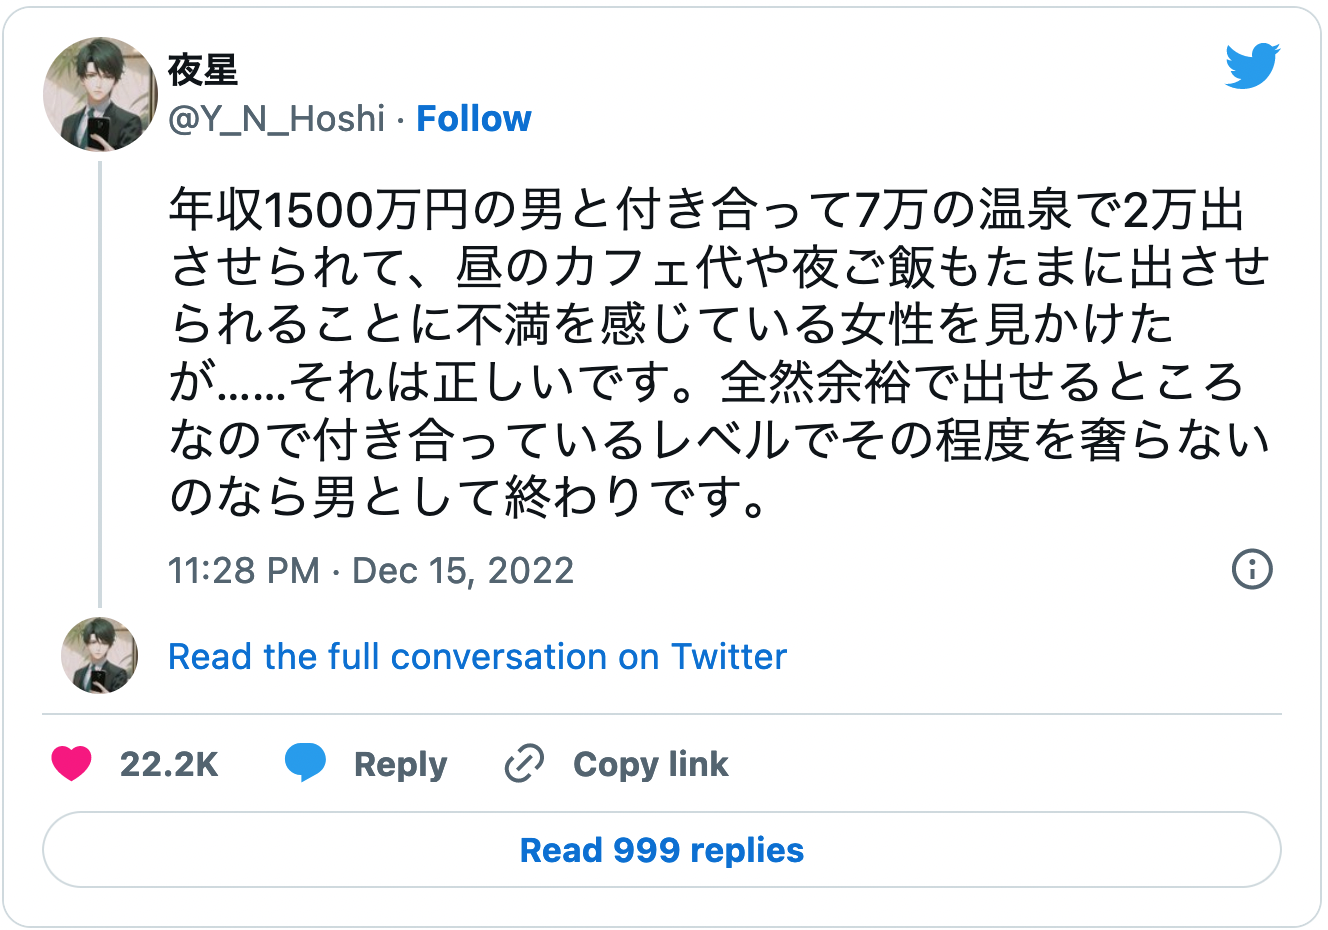
\includegraphics[width=0.85\textwidth]{./img/twitter.png}\cite{Y_N_Hoshi}
      \end{figure}
    \end{column}
    \begin{column}{0.3\textwidth}
      \simplecallout[{\LARGE\ce{:sunglasses:}}]{+}{green!10}{{\large\ce{:point_left:}これか!?}}
    \end{column}
  \end{columns}
\end{frame}

\begin{frame}
  \frametitle{奢り・割り勘問題}

  \begin{shadequote}[r]{}
    \begin{center}
      アリスとボブの飲食費について下記のいずれにするか決定する問題
      \begin{enumerate}
        \item ボブが全額を奢る
        \item 割り勘とする
      \end{enumerate}
    \end{center}
  \end{shadequote}

  \begin{columns}
    \begin{column}{0.5\textwidth}
      \centering
      \emph{アリス(Alice)}

      \begin{figure}[h]
        
\includegraphics[height=0.4\textheight]{img/alice.png}
      \end{figure}
    \end{column}
   
    \begin{column}{0.5\textwidth}
      \centering
      \emph{ボブ(Bob)}

      \begin{figure}[h]
        
\includegraphics[height=0.4\textheight]{img/bob.png}
      \end{figure}
    \end{column}
  \end{columns}
\end{frame}

\section{古典Covert Lottery}

\begin{frame}
  \frametitle{%
    カードを用いた古典Covert Lottery\protect\footnote{%
      \cite{covert_lottery_2021}では3人以上への拡張も踏まえてやや複雑な方法が説明されており、
      このプロトコルは発表者が2人を前提に独自に簡略化したものとなっている。%
    }
  }
  次のように物理的なカード\footnote{%
    これらのカードはトランプのようにいずれも裏が\commitedcard となっており、
    裏向きになった状態でどちらのカードなのか特定することができない。%
  }を用いて行う

  \pause
  \begin{columns}
    \begin{column}{0.6\textwidth}
      \begin{enumerate}
        \item アリス・ボブに2枚のカード\heartcard,\clubcard を配る
        \item アリス・ボブは表\ref{tbl:card_meaning}に従って
        希望を裏向き\commitedcard にして提出する\label{enum:cards_commited}

        \item \ballref{enum:cards_commited}で提出されたカードをシャッフルする
        
        \item どちらか1枚をドローして表向きにする \label{enum:result}
      \end{enumerate}

      \ballref{enum:result}のカードを表\ref{tbl:card_meaning}に対応させてプロトコルの結果とする
    \end{column}
    \begin{column}{0.4\textwidth}
      \begin{table}[h]
        \caption{カードの意味}
        \label{tbl:card_meaning}
        \begin{tabularx}{0.9\textwidth}{@{}| Y | Y |@{}}
          \hline
          カード & 意味 \\ \hline
          \heartcard & ボブの奢り \\ \hline
          \clubcard & 割り勘 \\ \hline
        \end{tabularx}
      \end{table}
    \end{column}
  \end{columns}
\end{frame}

\begin{frame}
  \frametitle{ケーススタディ\ballcircle{1} --- 2人の希望が一致}

  \pause
  \begin{itemize}
    \item<+-> 2人の希望が一致しているので次のようなケース
      \begin{columns}
        \begin{column}{0.5\textwidth}
          \alicecallout{+}{\heartcard}
        \end{column}
        \begin{column}{0.5\textwidth}
          \bobcallout{-}{\heartcard}
        \end{column}
      \end{columns}

    \item<+-> これらをシャッフルして1枚選んだときは必ず\heartcard となる

    \item<+-> 2人の希望が一致していればこのように必ずそちらが選ばれる
  \end{itemize}
\end{frame}

\begin{frame}
  \frametitle{ケーススタディ\ballcircle{2} --- 2人の希望が衝突}

  \begin{itemize}
    \item<+-> 2人の希望が衝突しているので次のようなケース
      \begin{columns}
        \begin{column}{0.5\textwidth}
          \alicecallout{+}{\heartcard}
        \end{column}
        \begin{column}{0.5\textwidth}
          \bobcallout{-}{\clubcard}
        \end{column}
      \end{columns}

    \item<+-> これらをシャッフルしてランダムに選べば、結果は\heartcard,\clubcard それぞれ$\frac{1}{2}$の確率になる
    \begin{description}
      \item[結果が\heartcard]<+-> アリスの希望どおり
      \item[結果が\clubcard]<+-> ボブの希望どおり
    \end{description}
    このように2つの結果がそれぞれ50\%のランダムとなる
  \end{itemize}
\end{frame}

\section{量子コンピュータとシュレディンガーの猫}

\begin{frame}
  \frametitle{量子コンピュータとシュレディンガーの猫}

  \begin{columns}
    \begin{column}{0.4\textwidth}
      \tableofcontents[currentsection]
    \end{column}
    \begin{column}{0.6\textwidth}
      \begin{itemize}
        \item このCovert Lotteryをカードではなくて量子コンピュータでやりたい

        \item その前にまずは量子コンピュータの基礎的なところを解説
      \end{itemize}
    \end{column}
  \end{columns}
\end{frame}

\begin{frame}
  \frametitle{量子コンピュータ}

  \begin{itemize}
    \item 古典コンピュータは1bitで\heartcard,\clubcard のような2つの値しか持たない

    \item 一方で量子コンピュータのbitに相当する\emph{qubit}は2つの複素数$c_0, c_1$によって次のように拡張される
    \begin{align}
      c_0\ket{\heartcard} + c_1\ket{\clubcard} \label{eq:qubit}
    \end{align}

    \item このとき$\ket{\heartcard}, \ket{\clubcard}$は$c_0, c_1$は次のようになる
    \begin{description}
      \item[$\ket{\heartcard}$] $c_0 = 1, c_1 = 0$
      \item[$\ket{\clubcard}$] $c_0 = 0, c_1 = 1$
    \end{description}

    % \item たとえば$\ket{\heartcard} = \Zero, \ket{\clubcard} = \One$のように行列で表せる
    % \[
    %   c_0\Zero + c_1\One = \left(
    %     \begin{array}{c}
    %       c_0 \\
    %       c_1
    %     \end{array}
    %   \right)
    % \]
  \end{itemize}
\end{frame}

\begin{frame}
  \frametitle{量子コンピュータ}

  \[
    c_0\ket{\heartcard} + c_1\ket{\clubcard} \tag{\ref{eq:qubit}}
  \]
  \begin{itemize}
    \item 式\ref{eq:qubit}の複素数$c_0, c_1$は\emph{確率振幅}と呼ばれ、
    次のように$\ket{\heartcard}, \ket{\clubcard}$が観測される確率を得ることができる
    \begin{description}
      \item[$\ket{\heartcard}$が観測される確率] $|c_0|^2$
      \item[$\ket{\clubcard}$が観測される確率] $|c_1|^2$
    \end{description}

    \item 確率なので、$c_0, c_1$は次の条件式\ref{eq:probability_amplitude_constraint}を満す
    \begin{align}
      |c_0|^2 + |c_1|^2 = 1 \label{eq:probability_amplitude_constraint}
    \end{align}

    \item 一方で$c_0, c_1$の具体的な値を直接知る方法はない
  \end{itemize}
\end{frame}

\begin{frame}
  \frametitle{ブロッホ球}

  \begin{columns}
    \begin{column}{0.6\textwidth}
      \begin{itemize}
        \item 複素数は実数$a, b$を用いて$a + b\sqrt{-1}$のように表現される
    
        \item 1qubitの表現に2つの複素数$c_0, c_1$が必要なので、4変数の自由度があるが
        下記2つの条件により\textbf{半径1の球の表面座標}と考えることができる
        \begin{enumerate}
          \item 確率の満す条件式\ref{eq:probability_amplitude_constraint}
          \item $c_0$が実数になるように$c_1$を調整してもいい
          (同じとみなせるqubitが存在する)
        \end{enumerate}

        \item この球のことを\textbf{ブロッホ球}と呼び、
        たとえば$\ket{\heartcard}$や$\ket{\clubcard}$はそれぞれ
        球の北極と南極の座標に対応する
      \end{itemize}
    \end{column}
    \begin{column}{0.4\textwidth}
      \begin{figure}
        \begin{blochsphere}[radius=0.4\textwidth, tilt=15,rotation=-20,opacity=0]
          \drawBallGrid[style={opacity=0.2}]{40}{40}
      
          \drawAxis[style={cyan}]{0}{0};
          \drawAxis[style={orange}]{90}{0};
          
          \labelLatLon{up}{90}{0};
          \labelLatLon{down}{-90}{90};
          \labelLatLon{left}{0}{0};
          \labelLatLon{right}{180}{0};
          \node[above] at (up) {$\ket{\heartcard}$};
          \node[below] at (down) {$\ket{\clubcard}$};
        \end{blochsphere}
        \caption{ブロッホ球}
      \end{figure}
    \end{column}
  \end{columns}
\end{frame}

\begin{frame}
  \frametitle{シュレディンガーの猫}

  \begin{columns}
    \begin{column}{0.4\textwidth}
      \begin{figure}
        \begin{blochsphere}[radius=0.38\textwidth, tilt=15,rotation=-20,opacity=0]
          \drawBallGrid[style={opacity=0.2}]{40}{40}
      
          \drawAxis[style={cyan}]{0}{0};
          \drawAxis[style={orange}]{90}{0};
          
          \labelLatLon{up}{90}{0};
          \labelLatLon{down}{-90}{90};
          \labelLatLon{left}{0}{0};
          \labelLatLon{right}{180}{0};
          \node[above] at (up) {$\ket{\heartcard}$};
          \node[below] at (down) {$\ket{\clubcard}$};
          \node[above] at (left) {$\ket{+}$};
          \node[above] at (right) {$\ket{-}$};
        \end{blochsphere}
        \caption{ブロッホ球上の$\ket{\pm}$}
      \end{figure}
    \end{column}
    \begin{column}{0.6\textwidth}
      \begin{itemize}
        \item ``シュレディンガーの猫''で有名なように、qubitは複素数を用いて
        次のようなブロッホ球の赤道上の座標を表現することもできる

        \item たとえば$c_0 = \frac{1}{\sqrt{2}}, c_1 = \pm\frac{1}{\sqrt{2}}$として
        次のような2つのqubitを考える
        \begin{align*}
          \ket{+} &\equiv \frac{1}{\sqrt{2}}\left(\ket{\heartcard} + \ket{\clubcard}\right) \\
          \ket{-} &\equiv \frac{1}{\sqrt{2}}\left(\ket{\heartcard} - \ket{\clubcard}\right)
        \end{align*}

        \item これらは$\ket{\heartcard}, \ket{\clubcard}$が観測される確率が
        いずれも$\left|\pm\frac{1}{\sqrt{2}}\right|^2 = \frac{1}{2}$になる
      \end{itemize}
    \end{column}
  \end{columns}
\end{frame}

\begin{frame}
  \frametitle{qubitの測定}

  \begin{itemize}
    \item 簡単のために、これまではqubitの測定は基底として$\left\{\ket{\heartcard}, \ket{\clubcard}\right\}$を
    前提としていた

    \item 実は直交基底(内積が$0$)であればよく、$\{\ket{+}, \ket{-}\}$でも測定ができる
  \end{itemize}
\end{frame}

\begin{frame}
  \frametitle{公平性の説明}

  \pause
  \begin{itemize}
    \item<+-> 参加者は送信する量子ビットを次の中から選択する
  \end{itemize}

  \begin{columns}
    \begin{column}{0.5\textwidth}
      \begin{table}[h]
        \footnotesize
        \begin{tabular}{|c|c|c|}
          \hline
          \diagbox{$a$}{$x$} & $0$       & $1$    \\ \hline
          $0$                & $\天国$    & $\地獄$ \\ \hline
          $1$                & $\生$      & $\死$  \\ \hline
        \end{tabular}
      \end{table}
    \end{column}
    \begin{column}{0.5\textwidth}
      \begin{figure}[h]
        \footnotesize
        \begin{blochsphere}[radius=0.15\textwidth, tilt=15,rotation=-20,opacity=0]
          \drawBallGrid[style={opacity=0.2}]{40}{40}
       
          \drawAxis[style={cyan}]{0}{0};
          \drawAxis[style={orange}]{90}{0};
           
          \labelLatLon{up}{72}{0};
          \labelLatLon{down}{-108}{90};
          \labelLatLon{left}{0}{0};
          \labelLatLon{right}{180}{0};
          \node[above] at (up) {$\天国$};
          \node[below] at (down) {$\地獄$};
          \node[above] at (left) {$\生$};
          \node[above] at (right) {$\死$};
        \end{blochsphere}
      \end{figure}
    \end{column}
  \end{columns}

  \begin{columns}
    \begin{column}{0.1\textwidth}
      \uncover<4->{
        
\includegraphics[width=\textwidth]{img/cat_russian_blue.png}
      }
    \end{column}
    \begin{column}{0.9\textwidth}
      \begin{itemize}
        \item<+-> 図のように$a$が同じ(= 色が同じ)なら直交する
       
        \item<+-> たとえば量子ビット$\地獄$の測定を考える
        \begin{description}
          \begin{columns}
            \begin{column}{0.4\textwidth}            
              \item[$\{\天国, \地獄\}$で測定した場合]\mbox{}\\
              常に$\地獄$が出力
            \end{column}
            \begin{column}{0.45\textwidth}           
               \item[$\{\生, \死\}$で測定した場合]\mbox{}\\
               $\生, \死$のいずれかが確率で出力
            \end{column}
          \end{columns}
        \end{description}
      \end{itemize}
    \end{column}
  \end{columns}
\end{frame}

\section{Quantum Covert Lottery}

\begin{frame}
  \frametitle{Quantum Covert Lottery}

  \begin{itemize}
    \item Quantum Covert Lotteryの説明

    \item Qiskitによるシミュレーション
  \end{itemize}
\end{frame}

\section{Covert Lotteryと情報リーク}

\begin{frame}
  \tableofcontents[currentsection]
\end{frame}

\begin{frame}
  \frametitle{コイントスとAND計算のハイブリッドプロトコル}

  \bobcallout{+}{%
    期待値的にはボブが不公平なままだが、\\
    もし不本意に奢った場合はアリスのがめつさが分かる
  }

  \pause
  \alicecallout{-}{%
    このときアリスはボブの奢りが本意か\\
    不本意か分からないが、奢られを得る
  }
\end{frame}

\begin{frame}
  \frametitle{コイントスとAND計算のハイブリッドプロトコル}

  \begin{columns}
    \begin{column}{0.6\textwidth}
      \uncover<+->{
        \alicecallout{+}{%
          逆にアリスが不本意に\\
          割り勘となってしまった場合、\\
          ボブの希望は割り勘だと特定する
        }
      }

      \uncover<+->{
        \bobcallout{-}{%
          しかしこのときボブは\\
          アリスの希望が分からない
        }
      }
    \end{column}
    \begin{column}{0.4\textwidth}
      \uncover<+(-2)->{
        \begin{itemize}
          \item アリスが不本意に割り勘となった場合、
          アリスは奢りを希望していたがボブは割り勘を希望しており、
          ランダムで割り勘となった

          \item<2-> このように希望通りになった側は相手の希望が分からず、
          希望通りにならかった側は相手の希望を知ることができる
        \end{itemize}
      }
    \end{column}
  \end{columns}
\end{frame}

\section{まとめ}

\begin{frame}
  \frametitle{まとめ}

  \pause
  \begin{itemize}
    \item<+-> 簡単なプロトコルで奢り・割り勘問題に決着をつけられるかもしれない
    \begin{itemize}
      \item 2人の参加者は安目・高目と情報を賭博する
    \end{itemize}

    \item<+-> 今回紹介した技術は``Covert Lottery\cite{covert_lottery}''という名前が付いている
    \begin{itemize}
      \item Covert Lotteryを量子コンピューターでやるという記事\cite{quantum_covert_lottery}を過去に書いた
    \end{itemize}

    \item<+-> 今回は2人だったが、これを多人数拡張すると別のゲームに使えるかも\ce{:thinking_face:}
  \end{itemize}
\end{frame}

\section*{参考文献}
\begin{frame}[allowframebreaks]
  \frametitle{参考文献}
  \nocite{*}
  \bibliographystyle{junsrt_url}
  \bibliography{ref}
\end{frame}

\begin{frame}
  \centering
  {\Huge Thank you for the attention!}
\end{frame}

\end{document}
